\documentclass[11pt]{article}
\usepackage[T1]{fontenc}
\usepackage[utf8]{inputenc}
\usepackage[a4paper,margin=2cm]{geometry}
\usepackage{graphicx}
\usepackage{enumitem}
\usepackage{booktabs}
\usepackage{parskip}
\usepackage{titlesec}
\usepackage{xcolor}

\setlist{nosep, leftmargin=1.4em}
\titlespacing*{\section}{0pt}{8pt}{4pt}
\titleformat{\section}{\large\bfseries}{\thesection.}{0.5em}{}
\pagenumbering{gobble}

\begin{document}

\begin{center}
{\LARGE\bfseries Ringkasan Eksekutif}\\[2pt]
{\large Model Mekanistik Reaksi Myristoylasi Insulin Detemir}\\[2pt]
\small 25 September 2026
\end{center}
\vspace{4pt}

\noindent\textbf{Inti singkat:} Tim R\&D telah membangun model komputer (model mekanistik)
yang mensimulasikan reaksi kimia pembentukan Insulin Detemir dari DesB30 di dalam reaktor,
termasuk pola pengadukan/pencampurannya, sehingga hasil (\emph{yield}) dan kemurnian produk
dapat diprediksi \textbf{sebelum} uji coba fisik dilakukan. Manfaat bagi pengambilan
keputusan: model ini memungkinkan pengujian perubahan proses secara komputasi lebih dulu,
sehingga mengurangi jumlah uji coba fisik yang mahal sebelum \emph{scale-up} ke skala pilot
maupun komersial. Akurasi model saat ini sudah cukup baik untuk penyaringan awal (\emph{go/no-go}),
namun \textbf{belum} cukup presisi untuk menetapkan spesifikasi final skala komersial.

\section{Apa yang Sudah Dikerjakan}
\begin{itemize}
  \item Model kinetika reaksi kimia (bagaimana DesB30 bereaksi dengan NHS-Myr menjadi
        Detemir), cocok dengan data eksperimen laboratorium.
  \item Model pencampuran (CFD -- simulasi aliran fluida) di dalam reaktor 5 L dan 250 mL,
        tervalidasi terhadap data eksperimen riil (selisih di bawah 0,1 satuan pH).
  \item Kedua model digabung menjadi satu model reaktor yang memprediksi hasil dan
        kemurnian pada kondisi operasi standar (SOP): NHS-Myr 0,482 mg/mL, laju alir pompa
        $\sim$12,96 mL/menit, dihentikan pada menit ke-30 $\rightarrow$ prediksi \textbf{64,8\%}
        yield Detemir, \textbf{71,9\%} kemurnian.
  \item Diuji secara independen (bukan hasil penyesuaian/\emph{fitting}) terhadap 2 batch
        produksi riil -- hasilnya berada dalam kisaran yang sama dengan prediksi:
\end{itemize}

\begin{center}
\small
\begin{tabular}{lccc}
\toprule
 & Konversi DesB30 & Yield Detemir & Kemurnian \\
\midrule
Prediksi model (SOP) & -- & 64,8\% & 71,9\% \\
Batch riil 1 & 95,06\% & 59,63\% & 62,73\% \\
Batch riil 2 & 94,83\% & 60,17\% & 63,45\% \\
\bottomrule
\end{tabular}
\end{center}

\begin{center}
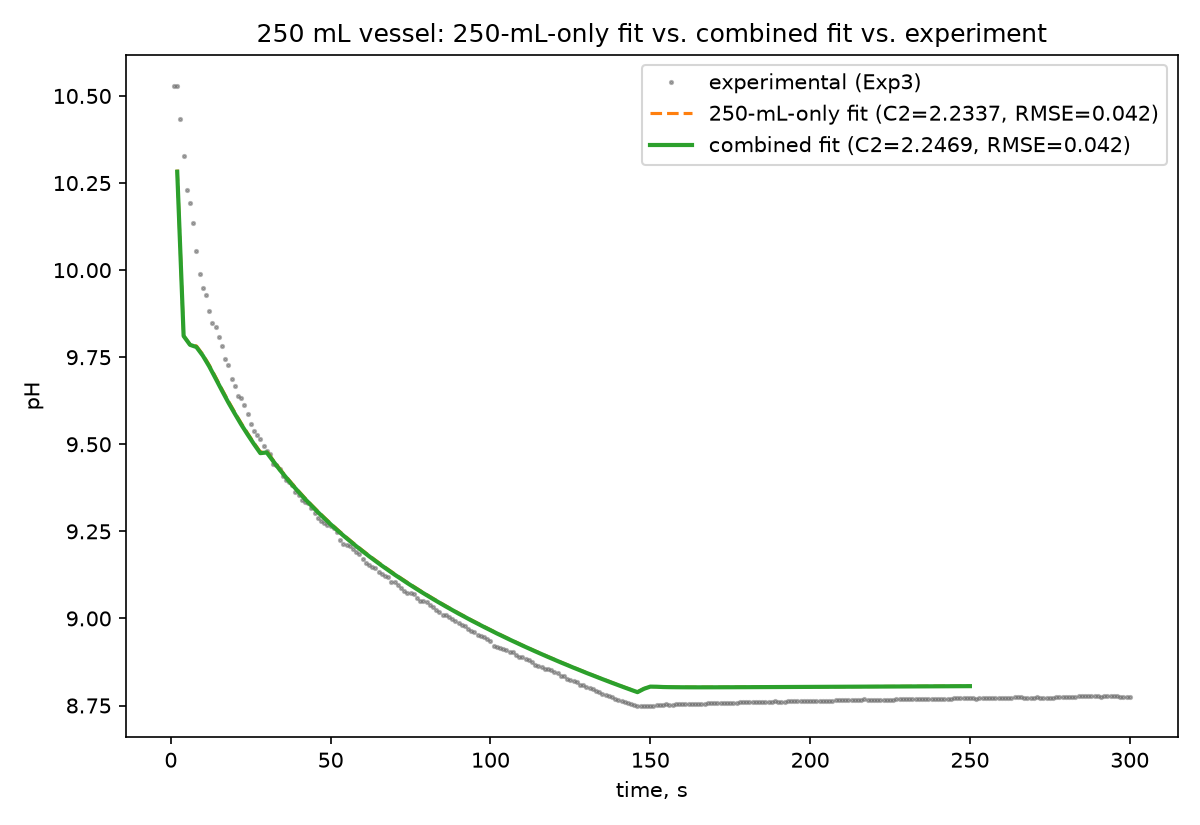
\includegraphics[width=0.62\linewidth]{figs_ringkasan/rans_5L_combined_fit_comparison.png}\\
{\footnotesize\itshape Model pencampuran (CFD) reaktor 5 L cocok dengan data eksperimen riil --
fondasi fisik model sudah tervalidasi.}
\end{center}

\section{Keterbatasan Saat Ini}
\begin{itemize}
  \item Baru diuji terhadap \textbf{2 batch} produksi riil -- belum cukup untuk klaim
        keandalan statistik yang kuat.
  \item Model saat ini memprediksi hasil/kemurnian sedikit lebih optimis
        ($\sim$5 poin persentase) dibanding 2 batch riil di atas.
  \item Sebagian konstanta laju reaksi (4 dari 10 parameter kinetika) belum sepenuhnya
        ``terkunci'' oleh data eksperimen yang ada -- rentang ketidakpastiannya masih lebar
        pada satu sisi.
  \item Model pencampuran baru tervalidasi pada skala laboratorium (250 mL dan 5 L) --
        \textbf{belum} pada skala komersial (3500 L).
\end{itemize}

\section{Data yang Perlu Dikumpulkan untuk Memperbaiki Model}
\begin{itemize}
  \item Data batch produksi riil tambahan (target minimal 5--6 batch, saat ini baru 2)
        untuk membangun rentang kepercayaan yang kuat secara statistik.
  \item Replikat eksperimen kinetika tambahan (saat ini 3 replikat per spesies) untuk
        mempersempit parameter yang masih longgar.
  \item Data sifat fisik cairan proses yang sesungguhnya (densitas, viskositas larutan
        Tris/HCl) dan pengukuran daya/torsi pengadukan aktual -- model pencampuran saat
        ini masih memakai asumsi sifat air murni dan batas literatur yang belum
        divalidasi langsung terhadap reaktor ini.
  \item Titik pengukuran kedua (mis. sensor pH di lokasi berbeda) pada eksperimen
        pencampuran, agar model CFD 3D penuh yang sedang direncanakan (di luar model
        sederhana saat ini) dapat divalidasi secara spasial, bukan hanya di satu titik --
        dan divalidasi pula pada skala menengah (pilot) atau komersial (3500 L)
        sebelum dipercaya penuh di skala tersebut.
\end{itemize}

\section{Apa yang Bisa Diharapkan Manajemen}
Dengan tiga perbaikan di atas, model dapat digunakan untuk menyaring keputusan proses dan
\emph{scale-up} secara komputasi -- mengurangi jumlah uji coba fisik yang mahal sebelum
komitmen ke skala komersial, sehingga \textbf{mempercepat waktu dari R\&D ke skala
komersial}.

\textbf{Skala dampak finansial:} Analisis biaya operasional (OPEX) terpisah untuk skala
komersial 3500 L (323 batch/tahun) menunjukkan target OPEX impas (\emph{break-even}) sebesar
Rp 634 juta/batch. Analisis tersebut juga menunjukkan bahwa faktor paling menentukan untuk
mencapai titik impas \textbf{bukan} penghematan sumber bahan baku semata, melainkan
\textbf{hasil (yield) per batch} -- menaikkan yield sekitar 30--50\% adalah pengungkit
terbesar menuju titik impas, jauh melebihi dampak penghematan pengadaan bahan baku. Yield
dan kemurnian adalah persis parameter yang diprediksi dan dioptimalkan oleh model
mekanistik ini -- sehingga model tersebut mendukung langsung keputusan finansial dengan
dampak terbesar di skala komersial.

\begin{center}
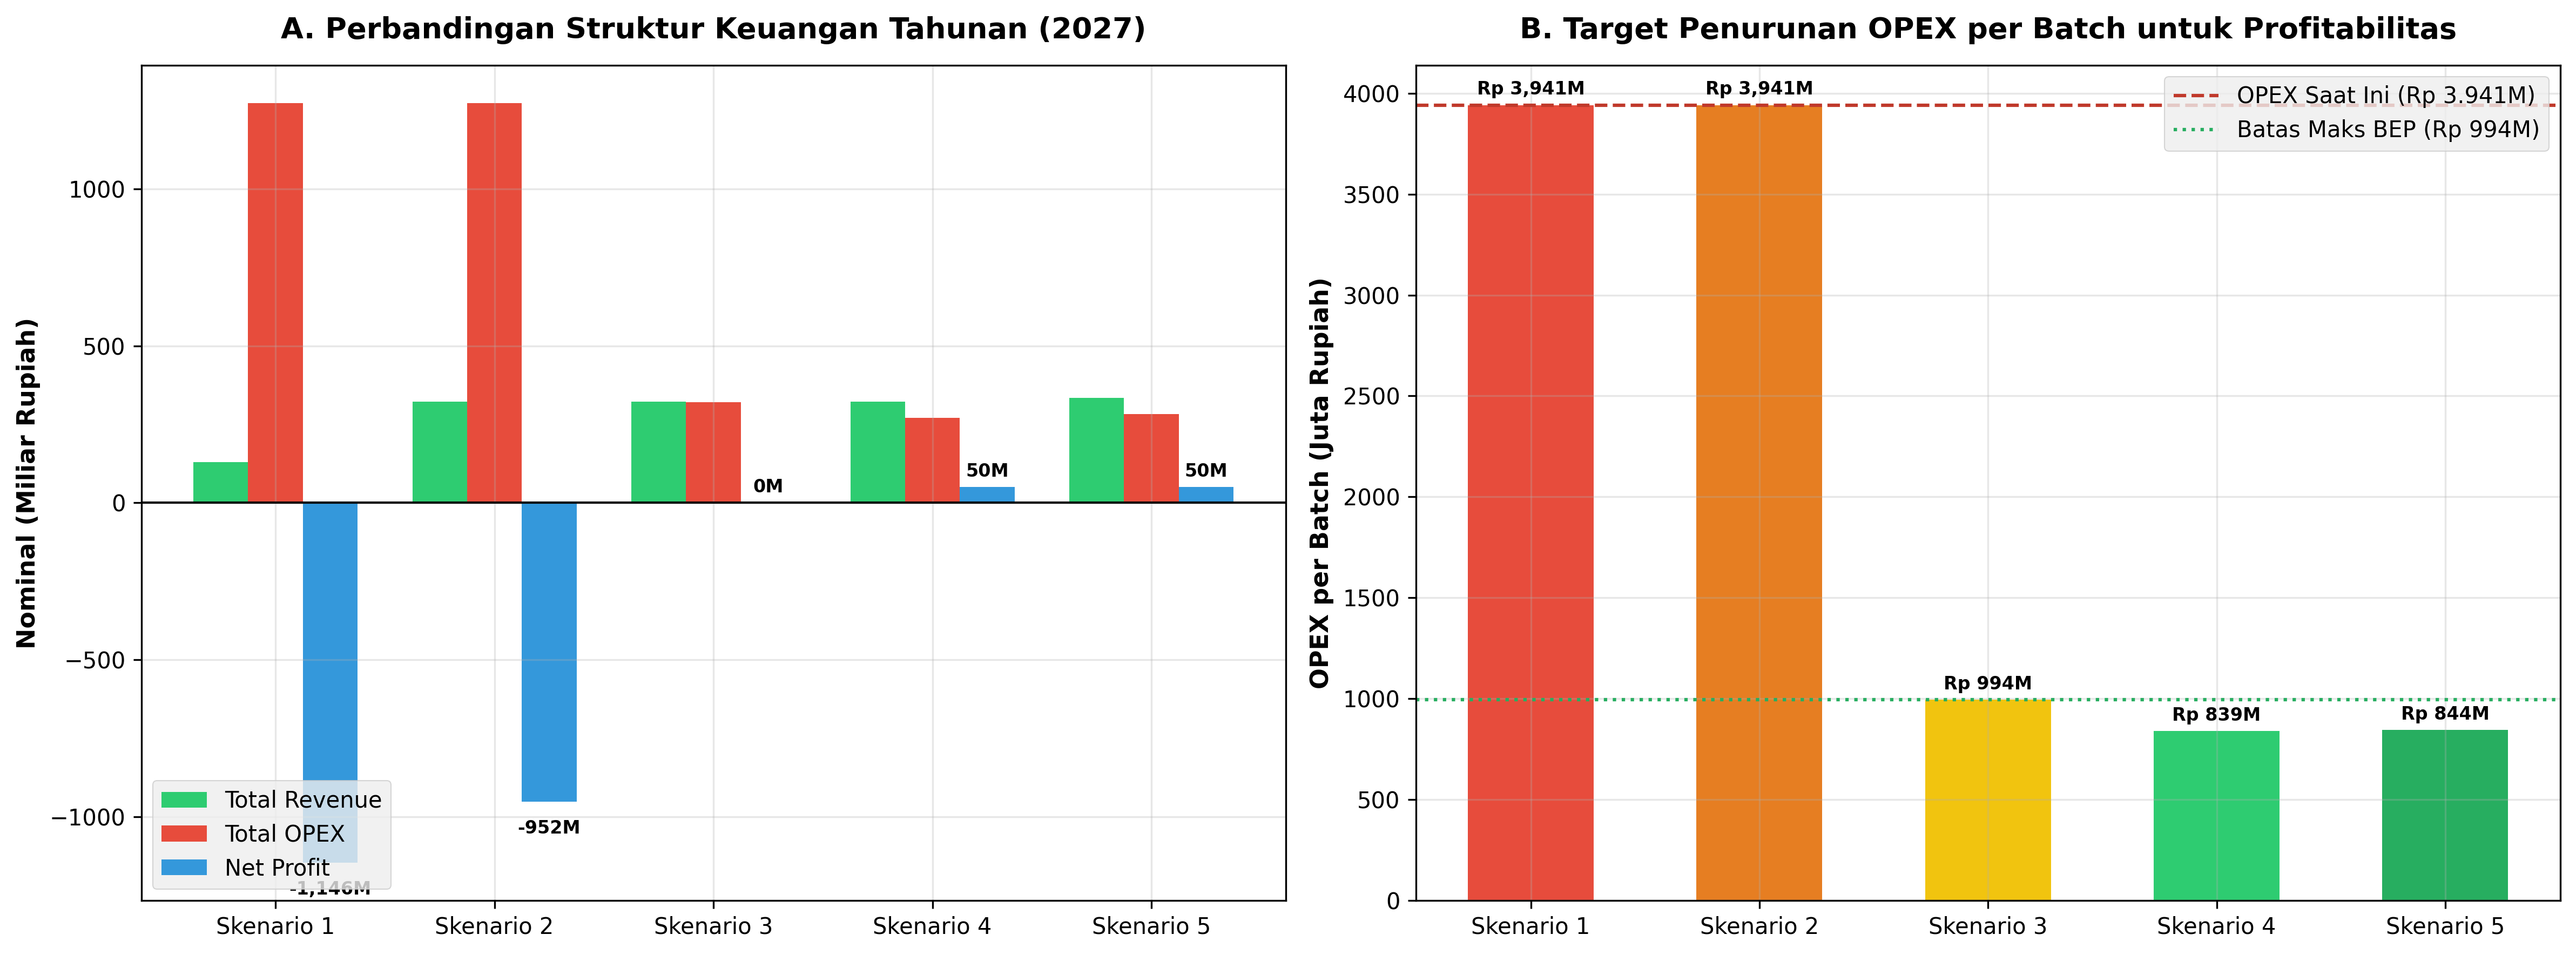
\includegraphics[width=0.6\linewidth]{figs_ringkasan/grafik_optimasi_profitabilitas.png}\\
{\footnotesize\itshape Skenario profitabilitas skala komersial (3500 L) -- yield adalah
pengungkit utama menuju titik impas.}
\end{center}

\noindent\textbf{Rekomendasi berikutnya:} (1) kumpulkan 3--5 data batch produksi riil
tambahan untuk memperkuat validasi model; (2) validasi model pencampuran pada skala
antara (pilot) sebelum berkomitmen penuh ke skala 3500 L.

\end{document}
